\documentclass[12pt]{article}

% --------- packages ---------
\usepackage{graphicx} % Required for inserting images
\usepackage{caption}
\usepackage{subcaption}
\usepackage{mleftright}
\usepackage{amsmath}
\usepackage{amsthm}
\usepackage{graphicx} % required for inserting images
\usepackage{multicol} % two column feature
\usepackage{etoolbox} % if-then-else logic
\usepackage{amsmath, amsfonts, amssymb, amsthm, mathrsfs} % math
\usepackage{complexity} % For \bigO and related commands
\usepackage{float} % figure env
\usepackage{tikz} % drawing things
\usetikzlibrary{automata, positioning,arrows.meta}
\usepackage{xcolor} % colors
\usepackage{transparent} % transparency
\usepackage[most]{tcolorbox} % answer boxes
\usepackage{fancyhdr} % header
\usepackage{fancyvrb} % fancy verbatim
\usepackage{ifthen} % conditional statements
\usepackage{lipsum} % filler text
\usepackage{xstring} % For string manipulation
\usepackage{enumitem} % for hint hanging indent
\usepackage[ruled,vlined]{algorithm2e} % algorithms

\newcommand{\bigO}{\mathcal{O}}

\title{CS3511 Final Project}
\author{Alex Chen, Adam Khalil, Dylan Zlatev, Arsheya Gourav}
\date{April 2025}

\begin{document}

\maketitle

Link to paper: https://arxiv.org/pdf/2104.01777

\section{Introduction}
While it may not seem like the order in which one multiplies a series of matrices makes much of a difference, the optimal ordering can reduce the number of scalar multiplications performed drastically, thus reducing the time it takes to multiply the matrices. However, doing so efficiently puzzled computer scientists for years, as they struggled to beat $\Theta(n^3)$ time bound. 

Finding an efficient solution to this problem would significantly improve numerous of its use cases, from speeding up compilers and tensor operations to enhancing the performance and image generation of GPUs that triangulate images to better render them \cite{Eberly}. Additionally, in database management using languages like SQL, a synonymous problem is the join-order problem, in which a SQL query with many joins uses a similar approach to MCM to find the optimal order of join operations \cite{Selinger}. Beyond the technological applications, MCM and PT algorithms are a staple in the dynamic programming section of any algorithms textbook. Thus, there is additional motivation to further explore and elaborate on this problem from a pedagogical perspective. 

The first major breakthrough that led closer to an efficient solution was the observation that the Matrix Chain Multiplication Problem is equivalent to the Polygon Triangulation problem, which aims to divide an $n$ sided polygon into $n-2$ triangles using $n-3$ lines, of which none can overlap, and while minimizing a cost associated with each vertex. 

While several papers described approaches to an efficient solution for the MCM and PT problems, such as a complex $\bigO(n\log n)$ PT solution by Hu and Shing and a simpler $\bigO(n^2)$ approach by Yao, the authors of this paper, Le and Gusfield, found the former too complex for classroom use and the latter lacking sufficient proofs. Therefore, in their paper, Le and Gusfield aimed to advance both the theory of these problems through an innovative, top-down branching search-tree algorithm, and the pedagogy of the topic by providing a digestible explanation and sufficient proofs for their worst-case time of $\Theta(n^2)$ approach. 

\section{Problem Statement \& Motivation}

Le and Gusfield has 5 main goals in their paper. Broadly, it aims to further both theory and algorithmic pedagogy:
\begin{enumerate}
    \item Simplify the findings of Yao in his paper where he developed and sketched a solution of the polygon triangulation problem. Yao was able to find a solution that runs in $\mathcal{O}(n^2)$ time. The revised proof aims to be more approachable for students in advanced algorithm classes.
    \item Generalize the $\mathcal{O}(n^2)$ solution and show that the time bound can be reached for $\textit{any}$ triangle-weight function that includes multiplicative and additive weighting.
    \item Show the $\textit{worst-case}$ running time of Yao's method, Le and Gusfield's version, is $\Theta(n^2)$.
    \item Show that the linear-time method with error bound of $15.5\%$ does not work in the additive-weight vairant of the polygon triangulation problem.
    \item Show that Le and Gusfield's variant of the algorithm runs in $\Theta(n \log n)$ time as opposed to Yao's $\Theta(n^2)$ on random data, illustrating the advantages of top-down memoization in comparison to bottom-up dynamic programming.
\end{enumerate}

\section{Technical Background}

The researchers provide technical background information to help demonstrate how the matrix-chain multiplication problem can be turned into a polygon triangulation problem to make the algorithm more efficient. 



In order to understand the findings of this paper it is crucial to understand polygon triangulation. Say we have a polynomial where all interior angles are less than 180°, this is a convex polygon. This polygon has $n$ nodes. Triangulation refers to the process of dividing the polygon into triangles by drawing non-crossing lines between corners. This results in $(n-2)$ triangles using $(n-3)$ non-crossing internal edges.

Now lets define a matrix chain problem to show how it translates to polygon triangulation:  $A_1 \times \cdots \times A_n$ with dimensions $d_0 \times d_1, \ldots, d_{n-1} \times d_n$. 

Every node (vertex) in the polygon will be defined as  $v_i$. Additionally, it is important to consider the weight of the nodes. Each vertex has a corresponding weight, $w_i$. Each triangle that makes up the polygon $\{v_i,v_j,v_k\}$ is the same thing as multiplying $(A_i \cdots A_j)(A_j \cdots A_k)$. This is because triangle weight $w_iw_jw_k$ equals multiplication cost $d_{i-1}d_jd_k$. The paper defines 3 different weight functions all used to minimize the number of scalar multiplications...



Multiplicative Weights: This is the weight of a triangle, the weight of each of its nodes multiplied together. This matches exactly how matrix multiplication costs are calculated.
\begin{equation}
f(v_i,v_j,v_k) = w_iw_jw_k \quad
\end{equation}
For example, say we are multiplying a 2×3 matrix with a 3×5 matrix (30 operations). And then we multiply the result (2×5 matrix) by a 5×7 matrix (70 operations). Polygon triangulation turns this into a problem where triangle weights (2×5×7) match up with multiplication costs (70), helping us find the cheapest order of multiplying.

Additive Weights: This is  simpler alternative optimization which optimizes how many times each node is used in triangles but does not directly translate to matrix costs. In this case, the weight of a triangle is the weight of all its nodes added.
\begin{equation}
f(v_i,v_j,v_k) = w_i + w_j + w_k \quad 
\end{equation}


Monotonicity Property: 
A weight function is monotonic if:
\begin{equation}
(w_i \leq w_i') \land (w_j \leq w_j') \land (w_k \leq w_k') \Rightarrow f(\cdot) \leq f(\cdot')
\end{equation}
What this means is that if the weight of a node is increased, the weight of the triangle will never increase. So both multiplicative and additive weights are monotonic.\\


The researchers make note of the \textbf{Theorem 1.1}: \\
This states that in order for a triangulation to be optimized (given that function $f$ is monotonic), the lightest node, $v_1$, must be connected to the second and third lightest nodes, $v_2$ and $v_3$. \\
Additionally, \textbf{Corollary 1.1} is stated and proven: \\
It addresses the case where $v_1$ is already adjacent to $v_2$ and $v_3$. In this case you either add an edge between $v_2$ and $v_3$ or add an edge between $v_1$ and the next lightest node, $v_4$. \\
 what is left: explain bridges and cones, talk about the existing algorithms to allow for comparison.

 Explained bridges and cones in solution section -Alex
\section{Solution}
With the above technical background in mind, Le and Gusfield propose a $O(n^2)$-time memoization algorithm to solve the polygon triangulation problem. Let us first introduce some key definitions:

Let $P(n, w)$ denote the original polygon for which we are trying to find the optimal triangulation of, with $n$ being the number of vertices and $w$ being the list of $n$ weights assigned to each vertex, and let $P$ be the current subproblem the algorithm is trying to solve. In other words, $P(n,w)$ denotes the polygon the algorithm is originally given as input, and $P$ denotes the sub-polygon the algorithm is currently trying to triangulate (since it is recursive). 

Let $v_i$ denote the $i$'th vertex of the current polygon $P$ with $i$'th smallest weight $w_i$. So $v_1$ would be the vertex with smallest weight in $P$, $v_2$ the vertex with second smallest weight, and so on.

With the above definitions in mind, we may begin discussing how Le and Gusfield's algorithm works on a high level. Polygons with three vertices (e.g., triangles) may be solved trivially by taking the product of the three vertex weights, so for the rest of this discussion we will assume that $P$ has at least four vertices.

The algorithm first determines in $P$ the three smallest vertices, $v_1$, $v_2$, and $v_3$. Note that there must be at least three vertices in $P$ as it is a polygon. Then, the algorithm may take one of three paths depending on how $v_2$ and $v_3$ are positioned relative to $v_1$ in $P(n,w)$ (not $P$).

Case 1: Exactly one of $v_2$ or $v_3$ is adjacent to $v_1$, and the other one is non-adjacent. In this case, the algorithm draws an internal edge from $v_1$ to whichever $v_2$ and $v_3$ is non-adjacent. This splits $P$ into two sub-polygons, which the algorithm then recurses on. This is shown in Fig. 1.

Case 2: Neither of $v_2$ or $v_3$ is adjacent to $v_1$. In this case, the algorithm draws internal edges from $v_1$ to both $v_2$ and $v_3$. This splits $P$ into \textit{three} sub-polygons, which the algorithm then recurses on. This is shown in Fig. 2.

Case 3: Both of $v_2$ and $v_3$ are adjacent to $v_1$. In this case, the algorithm branches into two possibilities, comparing them to see which yields the better outcome. In the first possibility, the algorithm draws an internal edge from $v_2$ to $v_3$. This splits $P$ into two sub-polygons, one of which is the triangle $\{v_1, v_2, v_3\}$. The algorithm recurses on each of these. In the second possibility, the algorithm draws an internal edge from $v_1$ to $v_4$. This splits $P$ into two sub-polygons, and the algorithm recurses on each of these. When both branches are solved, the algorithm compares the two and returns the one that is better. Overall, this case will create \textit{four} subproblems in total. This is shown in Fig. 3.

Although Case 1 and Case 2 both produce \textit{disjoint} subproblems, the issue in time complexity arises from Case 3, which produces two potentially \textit{overlapping} branches. This means that solving this problem without any additional tools will lead to a worst-case $\Theta(2^n)$ runtime. To resolve this issue, Le and Gusfield employ a dynamic programming approach using memoization. However, choosing how to represent a given subproblem in this dynamic programming representation requires some subtle and key insights about the nature of the algorithm. The researchers introduce two pieces of terminology: \textbf{bridges} and \textbf{cones}.

A bridge is a sub-polygon defined by an ordered pair $(v_i, v_j)$. It consists of the vertex $v_i$, all vertices on the clockwise walk from $v_i$ to $v_j$, and $v_j$. Bridges additionally have the following condition: on the aforementioned walk from $v_i$ to $v_j$, every vertex must have weight strictly greater than both $v_i$ and $v_j$. \textcolor{red}{Insert figure here}

A cone is a sub-polygon that can either be a bridge $(v_i, v_j)$, or a bridge $(v_i, v_j)$ plus an additional vertex $v_k$ such that $v_k$ has weight less than both $v_i$ and $v_j$. Thus, a cone can be represented by $(v_i, v_j, v_k)$, where $v_k$ is either some unambiguous filler value (we will use $-1$ if the cone is defined by just the bridge $(v_i, v_j)$, or a vertex with weight less than $v_i$ and $v_j$. Fig. 2 gives examples of both varieties of cone: the leftmost sub-polygon can be defined by the cone $(v_2, v_1, -1)$, and the middle sub-polygon by the cone $(v_3, v_2, v_1)$.

Finally, Le and Gusfield make the key assertion that every sub-polygon encountered during the execution of the algorithm can be represented by either a triangle (a solved subproblem) or a cone. Their proof for this is by induction, but is outside the scope of this report.

With this assertion, the total number of subproblems becomes nothing more than the total number of cones $(v_i, v_j, v_k)$. It may seem like there are $O(n^3)$ cones at first; however, note that $(v_i,v_j)$ must constitute a bridge, of Le and Gusfield show there are $O(n)$. Thus, there are actually only $O(n^2)$ cones in a given polygon. With some additional work showing that only constant work needs to be done each subproblem, the overall runtime of this polygon triangulation algorithm comes out to be $O(n^2)$.

\begin{figure}
\centering
\begin{minipage}{.5\textwidth}
  \centering
  \captionsetup{width=.8\linewidth}
  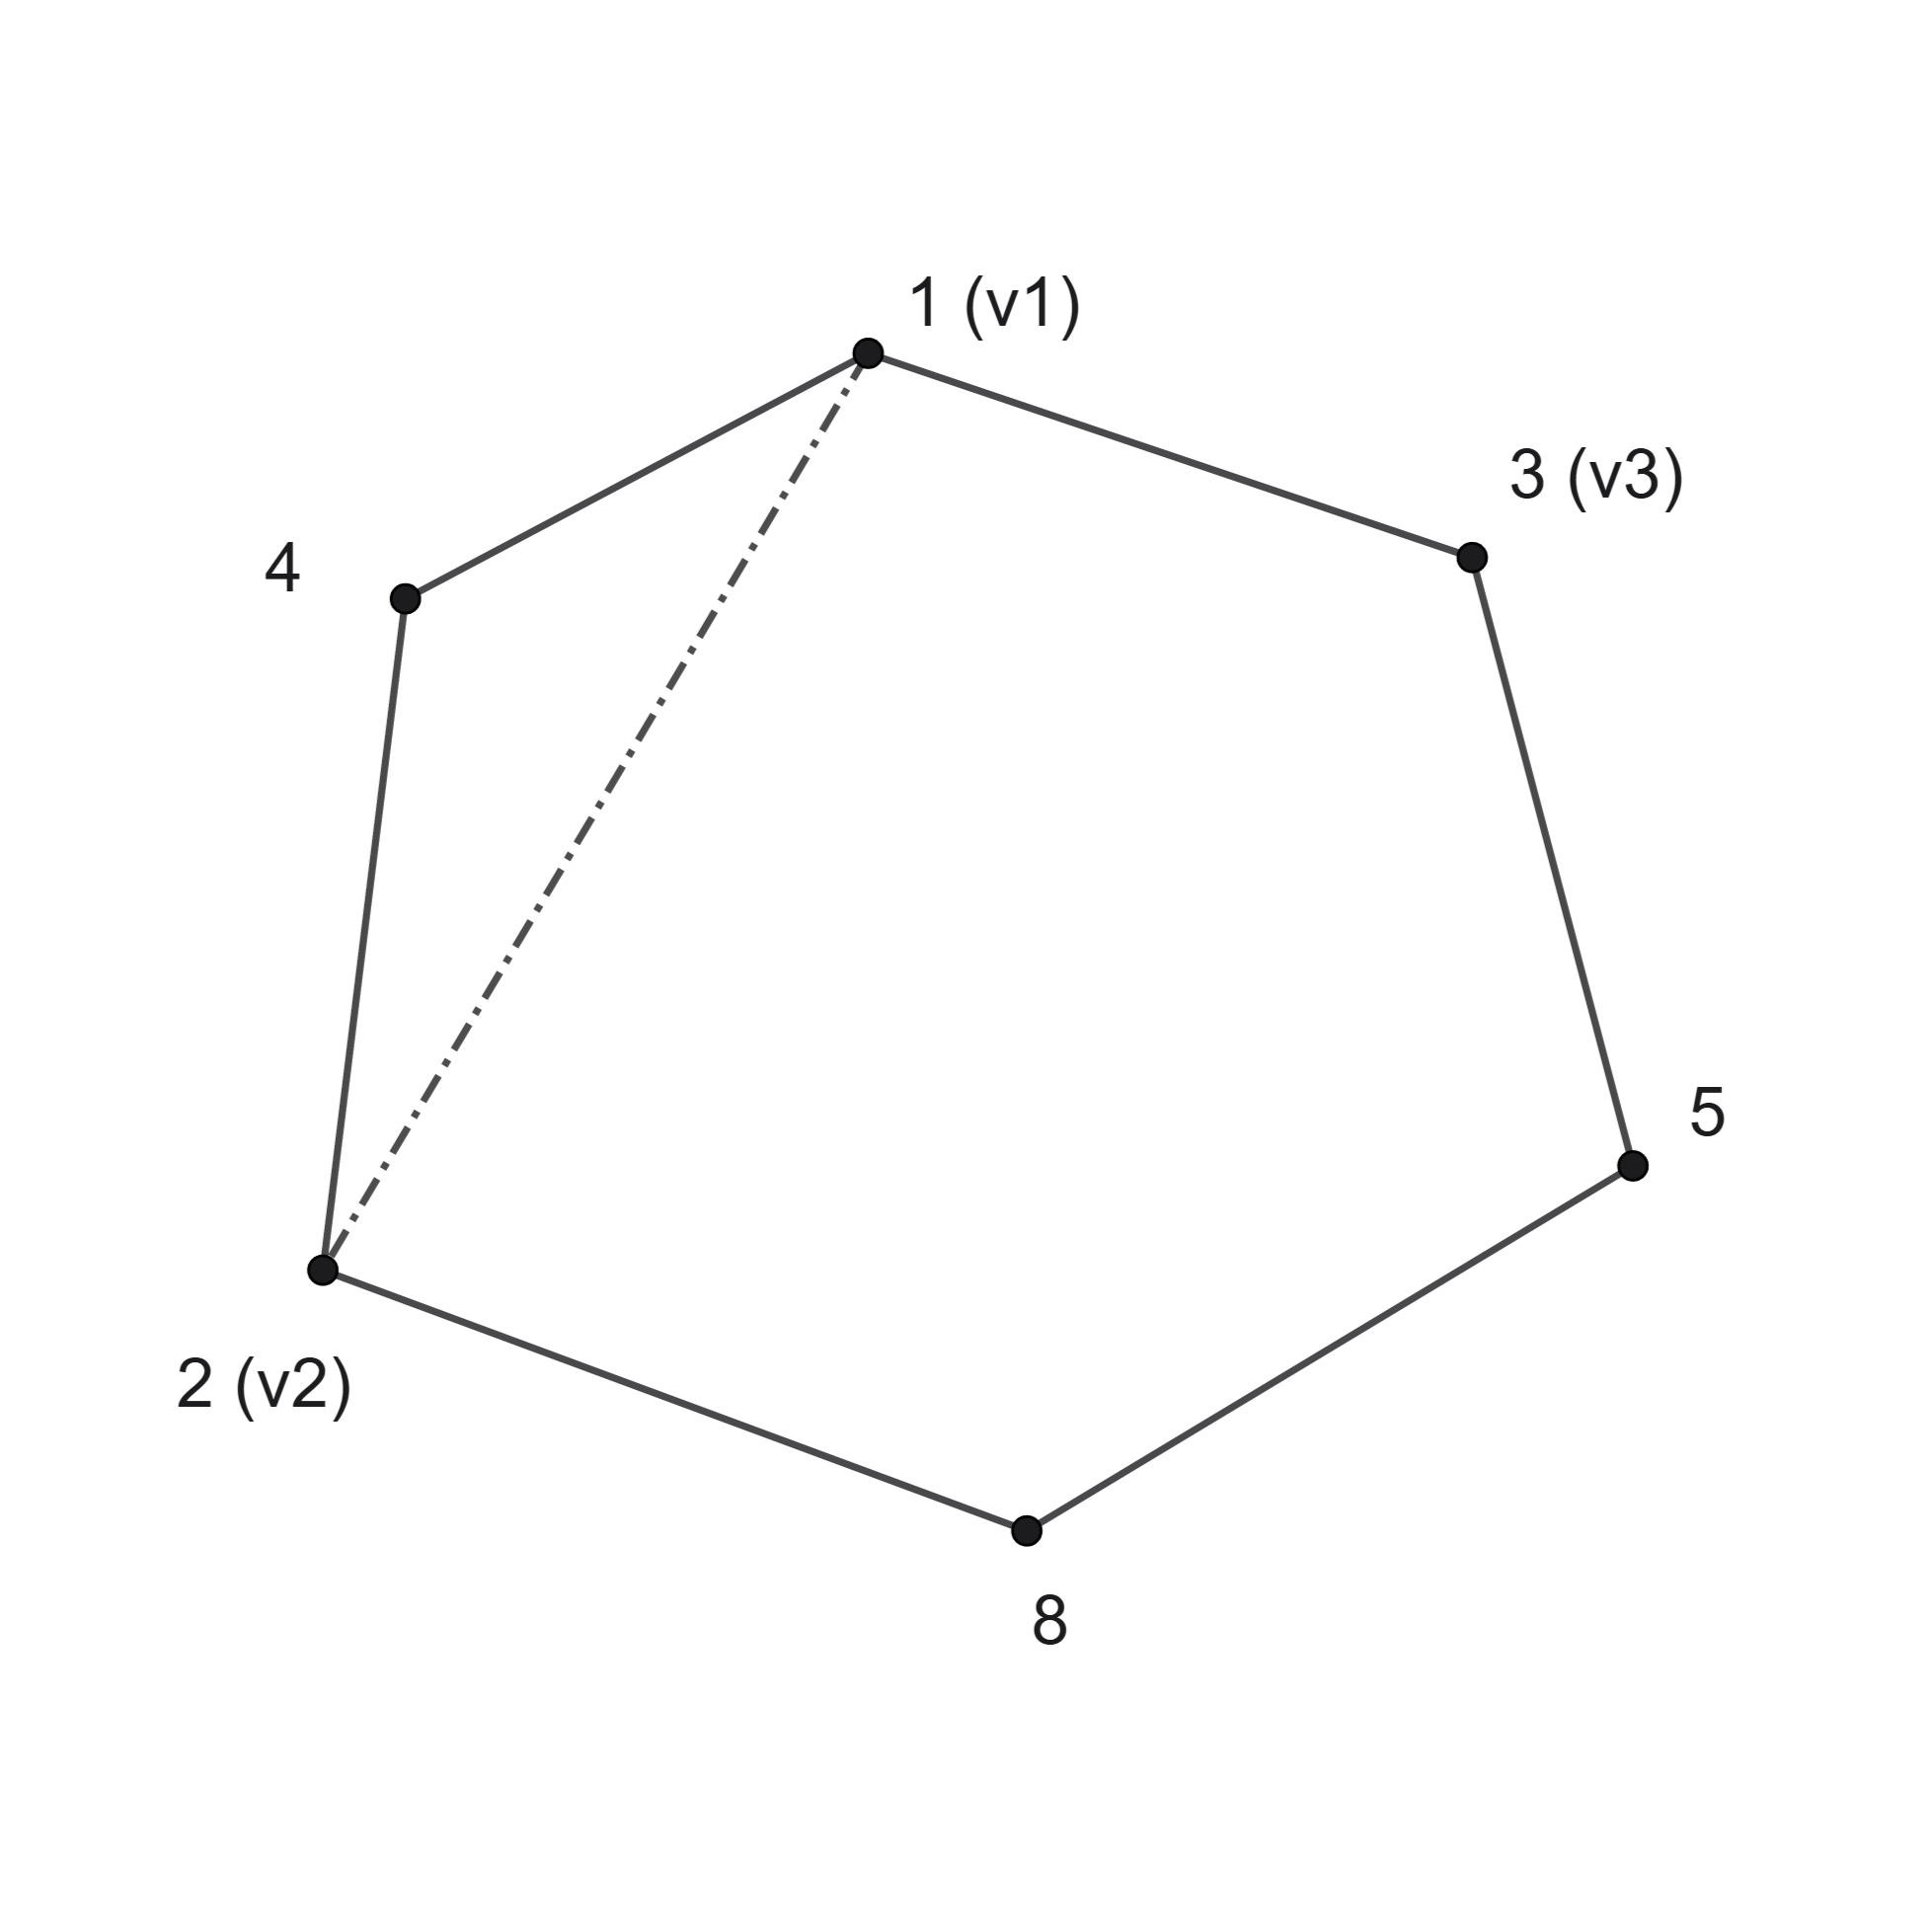
\includegraphics[width=\linewidth]{triangulation1.png}
  \captionof{figure}{Either $v_2$ or $v_3$ is not adjacent to $v_1$}
  \label{fig:test1}
\end{minipage}%
\begin{minipage}{.5\textwidth}
  \centering
  \captionsetup{width=.8\linewidth}
  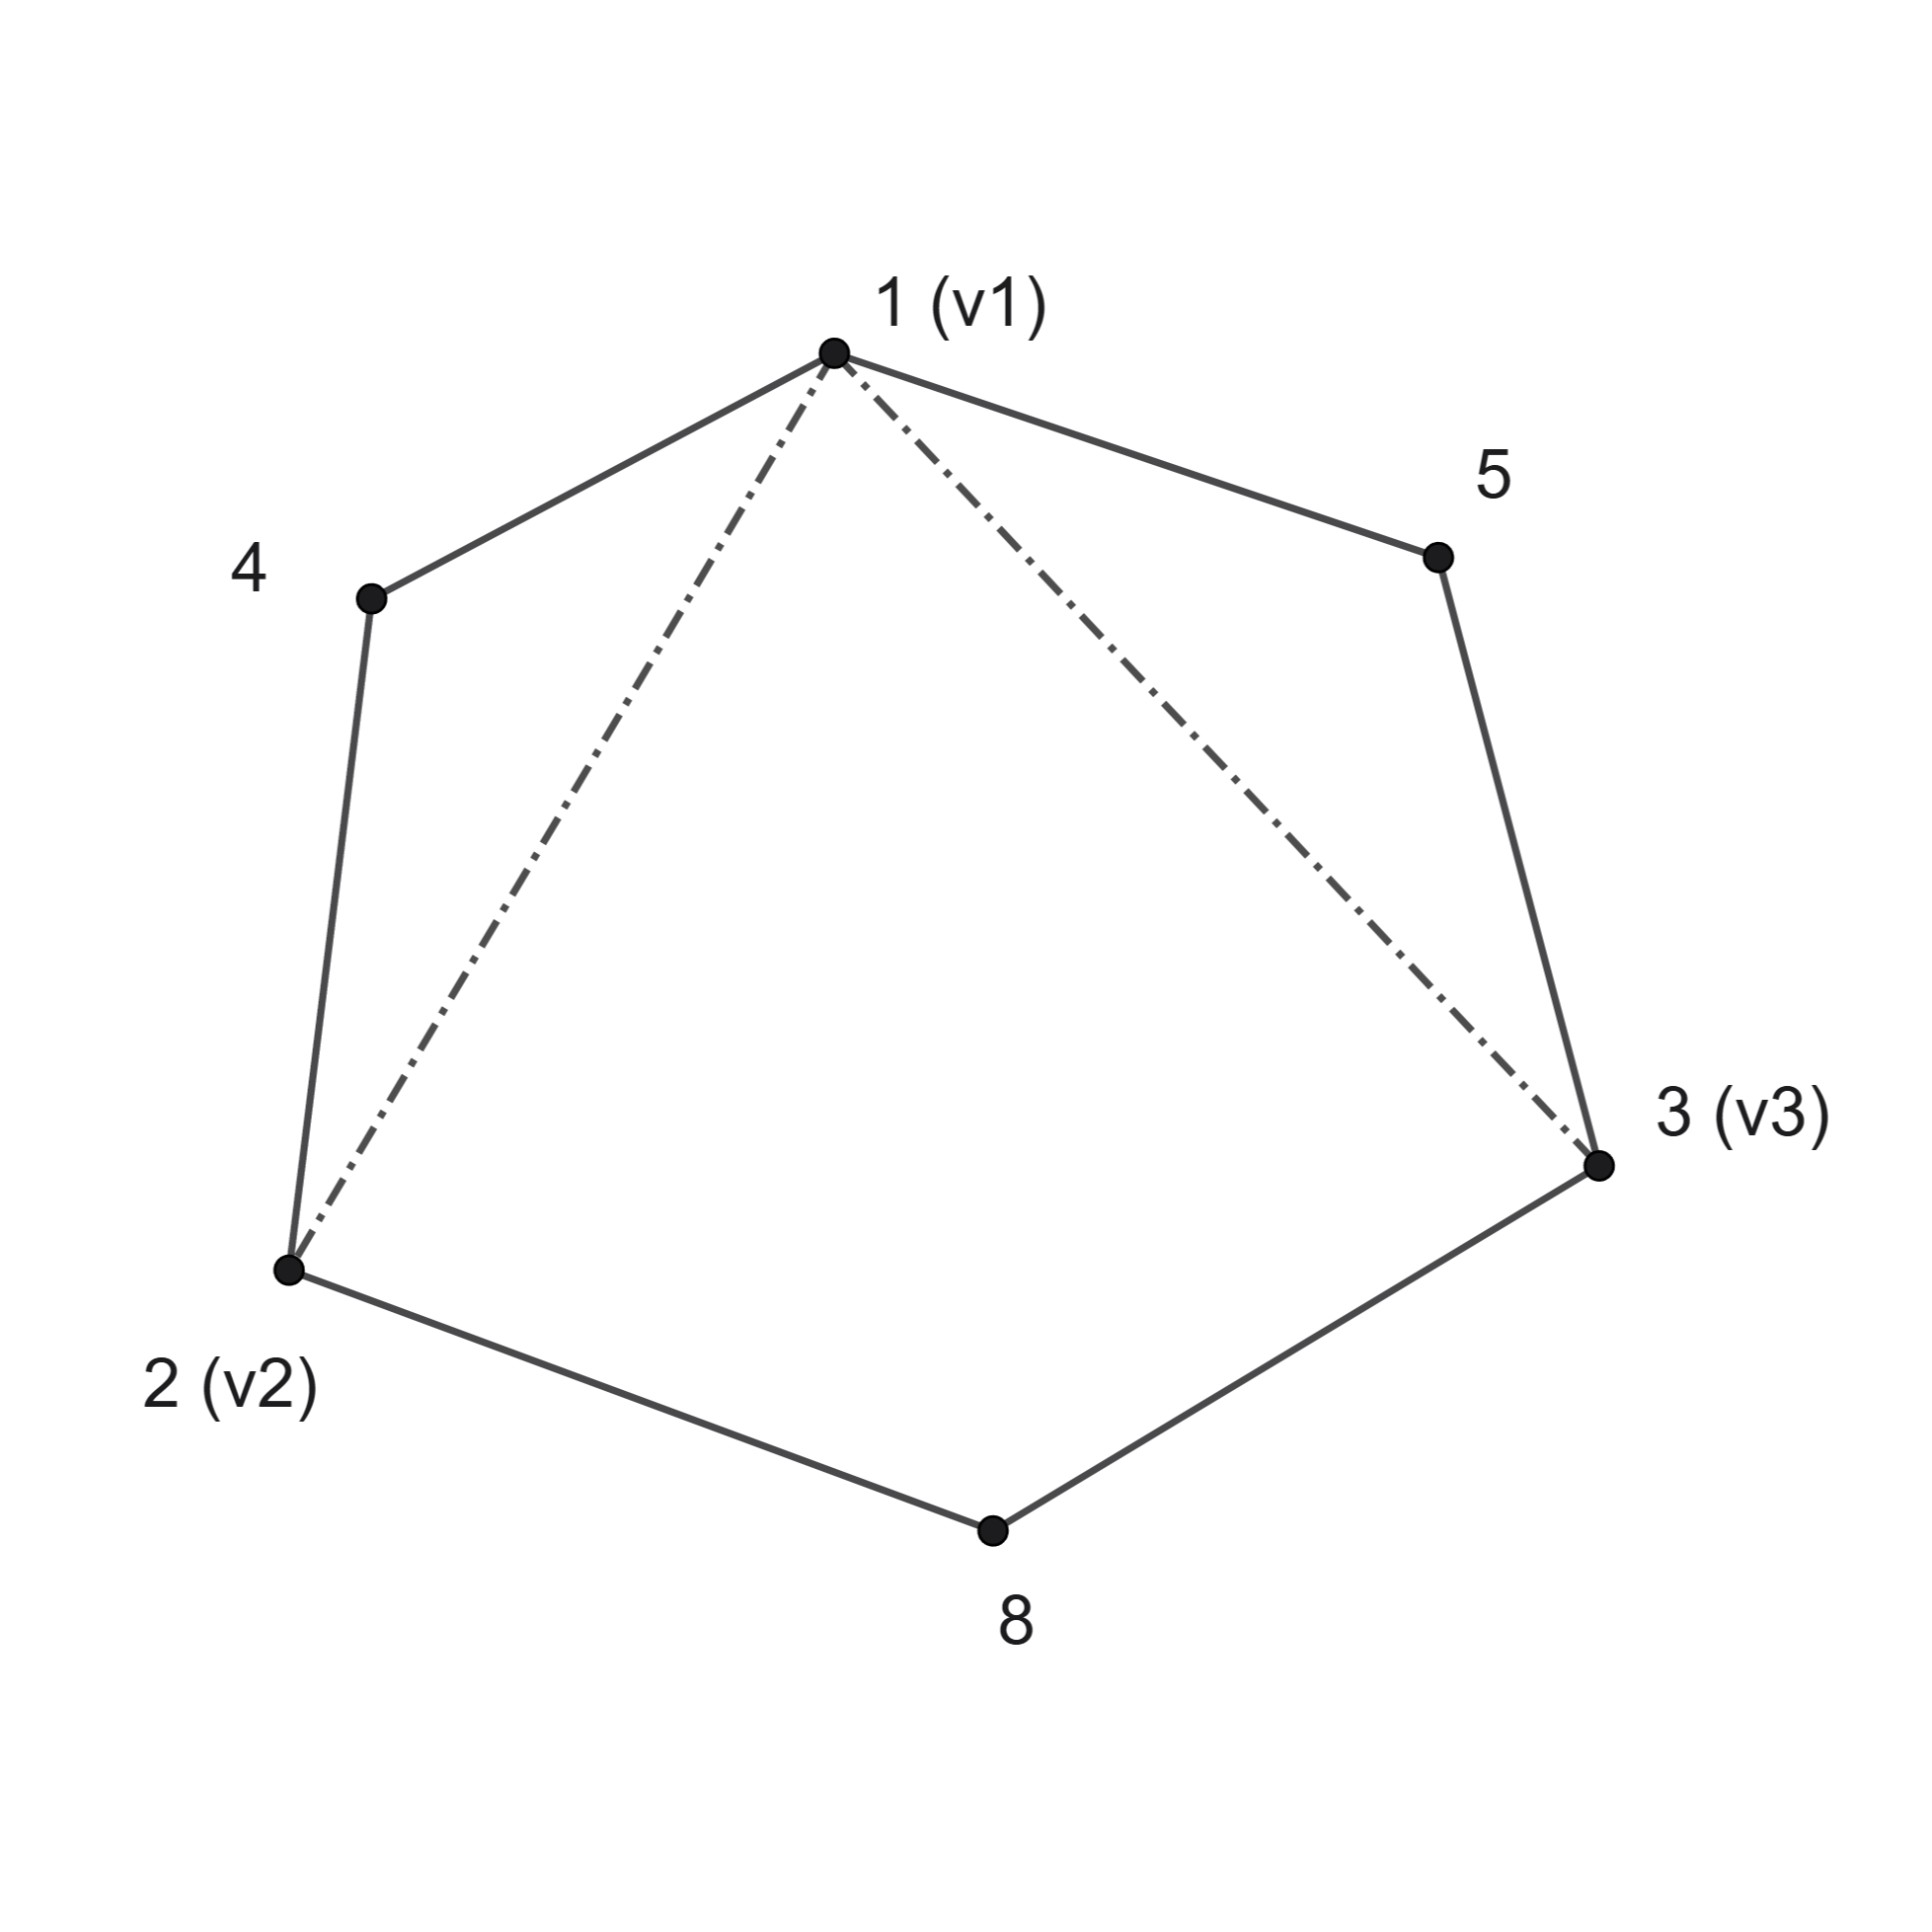
\includegraphics[width=\linewidth]{triangulation2.png}
  \captionof{figure}{Neither $v_2$ nor $v_3$ is adjacent to $v_1$}
  \label{fig:test2}
\end{minipage}
\end{figure}
\begin{figure}
\centering
\begin{subfigure}{.5\textwidth}
  \centering
  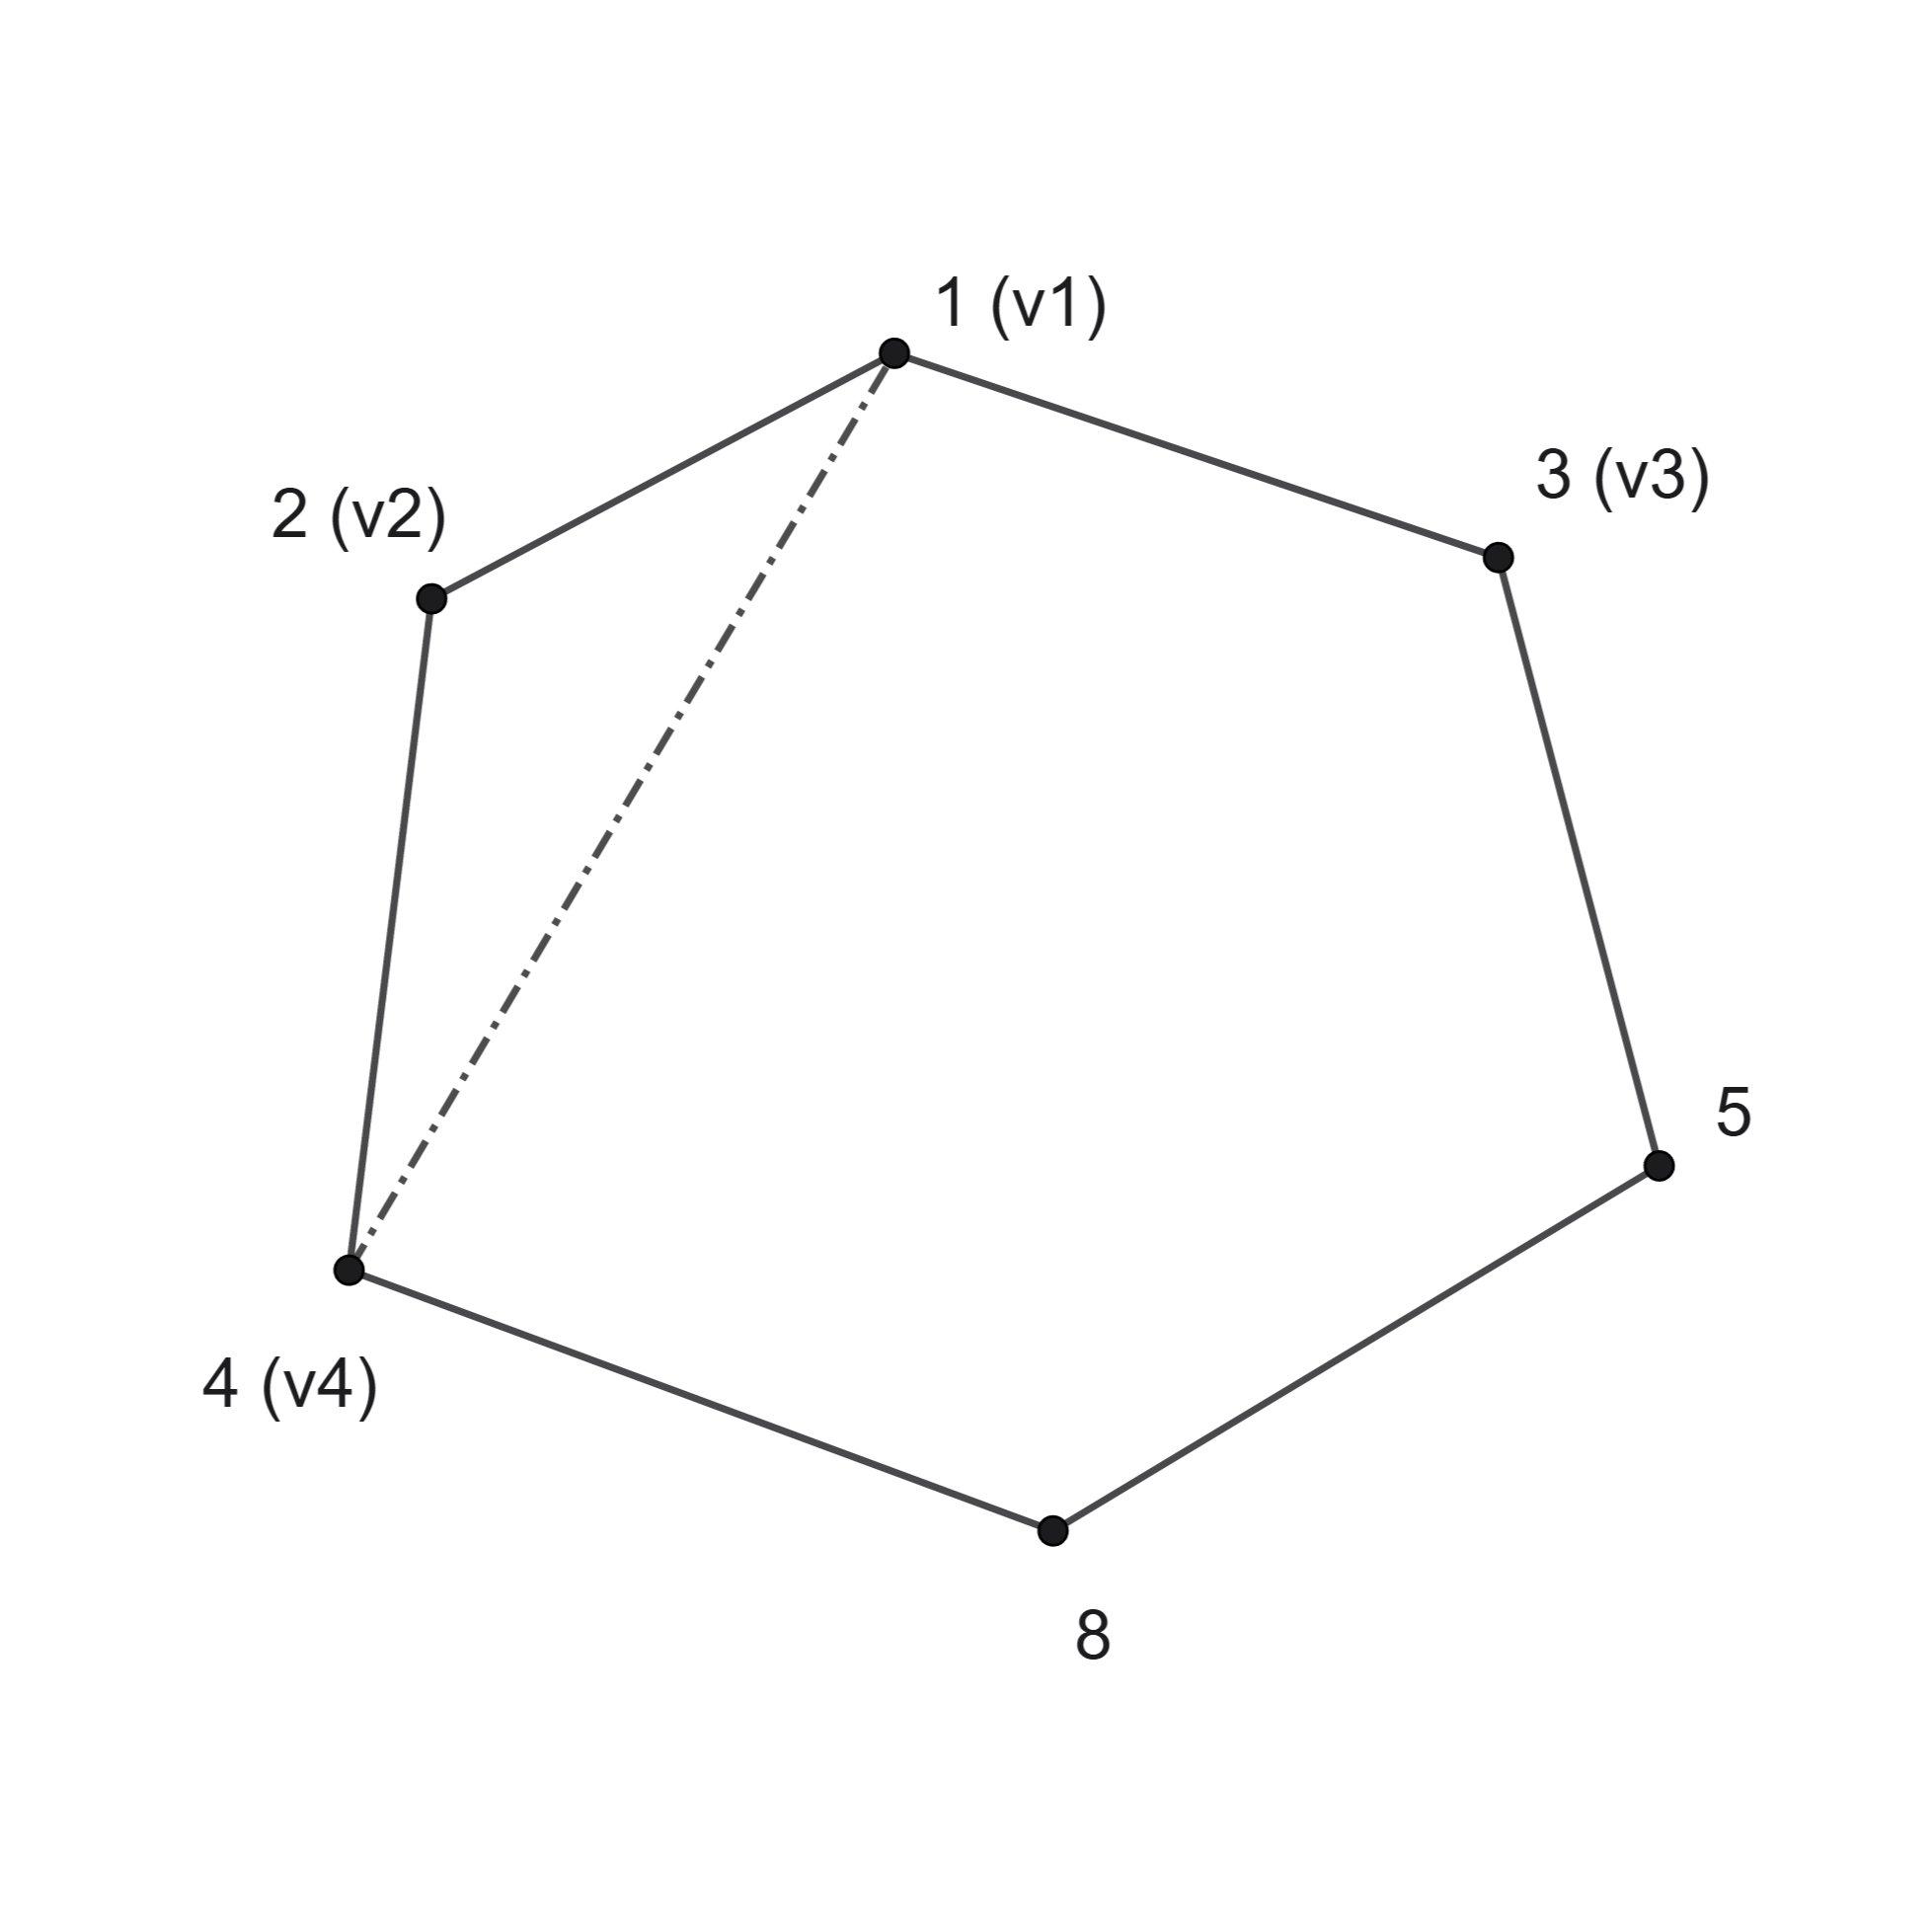
\includegraphics[width=\linewidth]{triangulation3a.png}
  \caption{Edge from $v_1$ to $v_4$}
  \label{fig:sub1}
\end{subfigure}%
\begin{subfigure}{.5\textwidth}
  \centering
  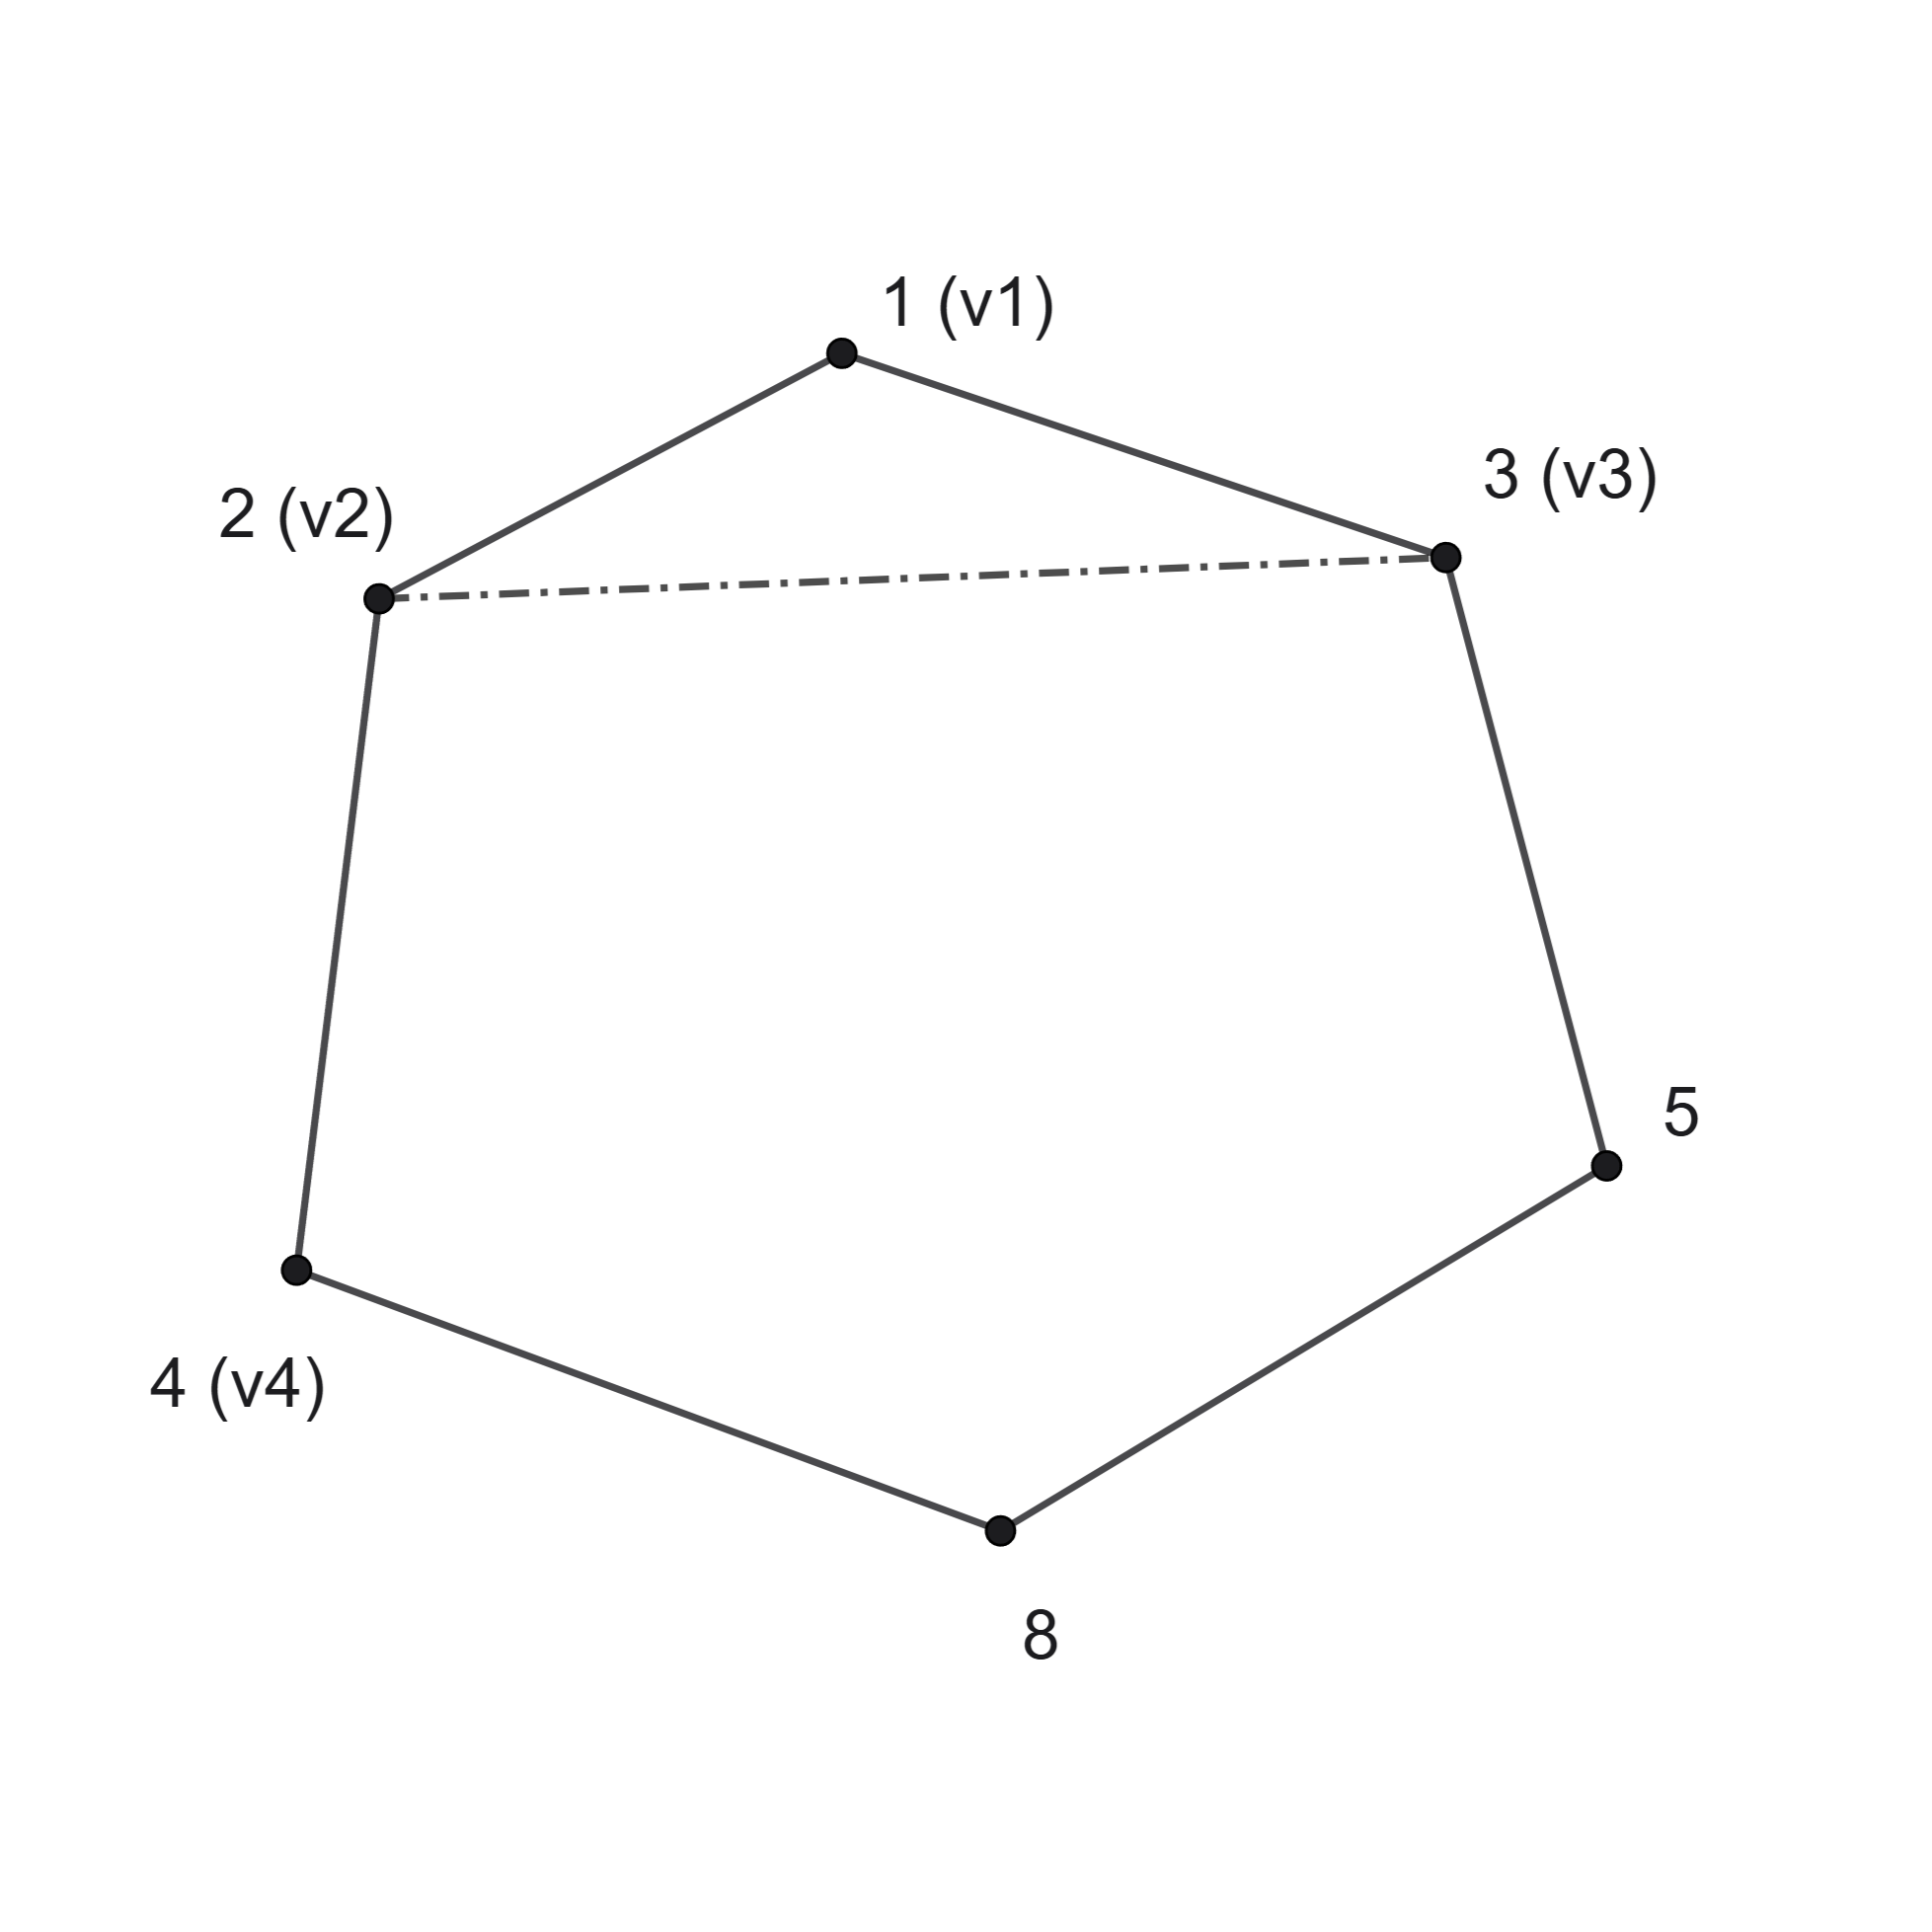
\includegraphics[width=\linewidth]{triangulation3b.png}
  \caption{Edge from $v_2$ to $v_3$}
  \label{fig:sub2}
\end{subfigure}
\caption{Both $v_2$ and $v_3$ are adjacent to $v_1$}
\label{fig:test}
\end{figure}


\section{Interactive Component/Conclusion}
In conclusion, this paper explained the Matrix Chain Multiplication (MCM) problem in the context of the equivalent Polygon Triangulation (PT) problem using a top-down branching search-trees approach. This method made use of several heuristics that allowed it to achieve a worst case runtime of $\bigO(n^2)$, and ran on random inputs in time $\Theta(n\log n)$, thus significantly outperforming the textbook $\bigO(n^3)$ method and outperforming Yao's $\Theta(n^2)$ approach in practice. 

The algorithms for the MCM and PT problems discussed in this paper can be further extended by representing the associated weights of each vertex of the PT problem as a probability distribution as opposed to a fixed weight \cite{Xiu}. This introduces the need to minimize the expected penalty of the algorithm instead, and is more applicable to real settings such as database management and compiler optimization, where the cost statistics typically vary randomly and do not have a fixed nature. 


\textbf{Idea for Interactive Component:}\\
We plan to implement a visualization of this in code and are currently working on it in our shared Github repo.


\begin{thebibliography}{99}          % 99 = widest label

\bibitem{Eberly}
Eberly, “Triangulation by Ear Clipping” (\emph{Tech. Rep}. 2002, last rev. 2024)

\bibitem{LeGusfield2021}
Thong~Le and Dan~Gusfield.
Matrix Chain Multiplication and Polygon Triangulation Revisited and
Generalized.
\emph{CoRR}, abs/2104.01777, 2021.

\bibitem{Selinger}
Selinger et al. “Access Path Selection in a Relational DBMS” (\emph{ACM} ’79).

\bibitem{Xiu}
Haibo Xiu, Pankaj K. Agarwal, and Jun Yang.
“PARQO: Penalty‑Aware Robust Plan Selection in Query Optimization.”
Proceedings of the VLDB Endowment 17 (2024), 4627‑4640.


\end{thebibliography}

\end{document}
